%% LyX 2.0.2 created this file.  For more info, see http://www.lyx.org/.
%% Do not edit unless you really know what you are doing.
\documentclass[twoside,twocolumn,french]{paper}
\renewcommand{\familydefault}{\sfdefault}
\usepackage[T1]{fontenc}
\usepackage[utf8]{inputenc}
\usepackage[a4paper]{geometry}
\geometry{verbose,tmargin=2cm,bmargin=2cm,lmargin=2cm,rmargin=2cm}
\pagestyle{plain}
\setcounter{tocdepth}{2}
\setlength{\parskip}{\smallskipamount}
\setlength{\parindent}{0pt}
\usepackage{babel}
\addto\extrasfrench{%
   \providecommand{\og}{\leavevmode\flqq~}%
   \providecommand{\fg}{\ifdim\lastskip>\z@\unskip\fi~\frqq}%
}

\usepackage{float}
\usepackage{graphicx}
\usepackage[unicode=true,pdfusetitle,
 bookmarks=true,bookmarksnumbered=false,bookmarksopen=false,
 breaklinks=false,pdfborder={0 0 1},backref=section,colorlinks=false]
 {hyperref}

\makeatletter
%%%%%%%%%%%%%%%%%%%%%%%%%%%%%% User specified LaTeX commands.
\usepackage{babel}
\setlength{\columnsep}{1.3cm}

\makeatother

\begin{document}

\title{Planteuse traine-fesses}


\institution{ADABio-Autoconstruction}

\maketitle
\href{http://www.adabio-autoconstruction.org/outils/tous-les-outils/planteuse-traine-fesses-v-1-0.html}{URL}
\begin{abstract}
L’outil présenté ici et surnommé « Traine-fesses » permet de gagner
un temps précieux lors de la plantation. Un rouleau traceur marque
l’emplacement pour la plantation, un cadre présente les caisses de
légumes aux opérateurs qui sont assis au ras du sol et n’ont plus
qu’à planter au bon endroit.
\end{abstract}
Nous vous présentons la v.1.0 de l’assistant de plantation \textquotedbl{}traine-fesses\textquotedbl{},
un système inspiré notamment de matériels recensés sur l’exploitation
de Franck Vuillermet à Chambéry.

Cette version n’est pas définitive. Elle réclame au contraire vos
commentaires, idées et modifications.

\begin{figure}[H]
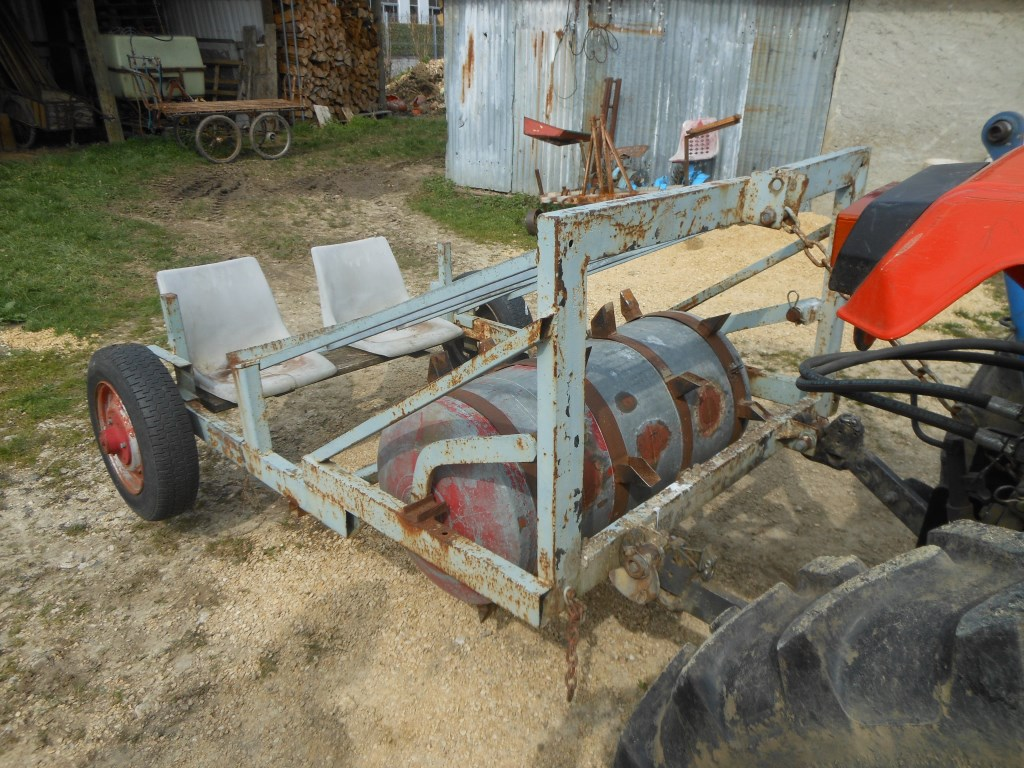
\includegraphics[width=1\columnwidth]{files/dscn2789}

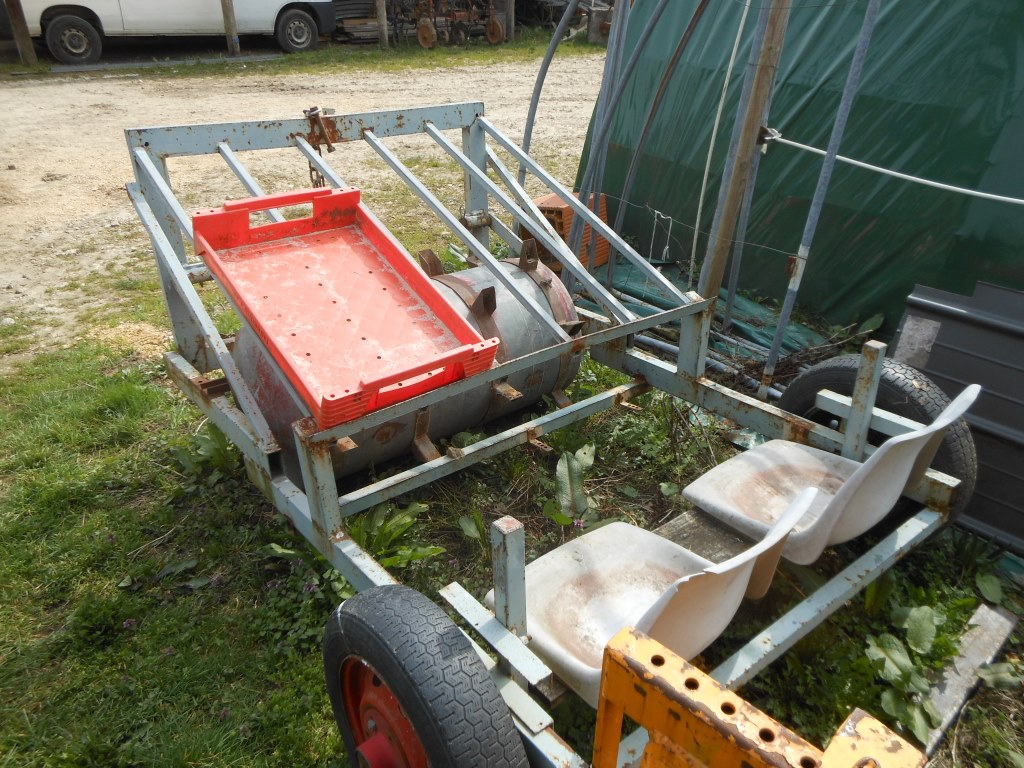
\includegraphics[width=1\columnwidth]{files/dscn2791}

\caption{L’original de Franck Vuillermet sans le triangle d’attelage}
\end{figure}



\section*{Liens}

\href{http://www.adabio-autoconstruction.org/IMG/pdf/tutoriel_traine-fesses_3.pdf}{tutoriel assistant de plantation v.1.0}

\href{http://forum.adabio-autoconstruction.org/viewtopic.php?f=51&t=2166}{forum.}
\end{document}
